% ICPR 2026 Manuscript Template
% Based on Springer LNCS format
%
\documentclass[runningheads]{llncs}
%
\usepackage[T1]{fontenc}
\usepackage{graphicx}
%
\begin{document}
%
\title{Paper Title\thanks{Supported by [funding source].}}
%
\author{First Author\inst{1}\orcidID{0000-0000-0000-0000} \and
Second Author\inst{2}\orcidID{0000-0000-0000-0000}}
%
\authorrunning{F. Author et al.}
%
\institute{[Institution 1], [Address], [Country]
\email{[email]@domain} \and
[Institution 2], [Address], [Country]
\email{[email]@domain}}
%
\maketitle
%
\begin{abstract}
[Abstract placeholder. Briefly summarize the contents of the paper in 150--250 words.]

\keywords{Keyword 1 \and Keyword 2 \and Keyword 3}
\end{abstract}
%

\section{Introduction}
%
[Introduction placeholder. State the problem, motivation, and contributions.]

%

\section{Related Work}
%
[Related work placeholder. Survey and discuss relevant prior work.]

%

\section{Method}
%
[Method placeholder. Describe your approach, model, or algorithm.]
%
\subsection{Overview}
[Subsection placeholder.]
%
\subsection{Implementation Details}
[Implementation details placeholder.]

%

\section{Experiments}
%
[Experiments placeholder. Describe setup, datasets, and evaluation protocol.]
%
\subsection{Experimental Setup}
[Setup placeholder.]
%
\subsection{Results}
[Results placeholder. Add tables and figures as needed.]
%
% Example figure (uncomment when ready):
% \begin{figure}
% 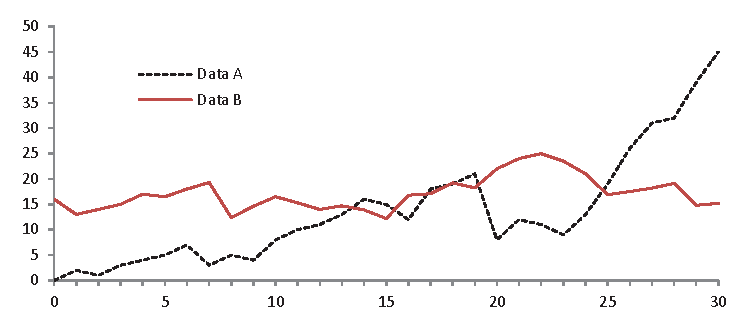
\includegraphics[width=\textwidth]{fig1.eps}
% \caption{Figure caption.} \label{fig1}
% \end{figure}

%

\section{Conclusion}
%
[Conclusion placeholder. Summarize contributions and future work.]

%
% ---- Bibliography ----
% Use splncs04 style for BibTeX, or maintain references below manually.
%
% \bibliographystyle{splncs04}
% \bibliography{references}
%
\begin{thebibliography}{8}
\bibitem{ref1}
[Add references here.]
\end{thebibliography}
\end{document}
